% ==============================================================================
% Section 9: Independence & Conditional Coverage: Christoffersen Backtesting
% Target: Page 11 (Exactly 1 Page)
% ==============================================================================

\section{Independence and Conditional Coverage: Christoffersen Backtesting}
\label{sec:christoffersen_backtesting}

\subsection{The Blindness of Unconditional Backtesting to Breach Clustering}

The Kupiec POF test evaluates only total exceptions, remaining completely indifferent to their temporal clustering \citep{christoffersen1998evaluating}. In banking practice, consecutive breaches induce acute liquidity strain. To ensure risk models adapt dynamically, model validation requires testing for **exception independence**.

\subsection{Markov Chain Formulation and Independence Likelihood Ratio}

\citet{christoffersen1998evaluating} modeled the exception sequence $\{I_1, \dots, I_N\}$ as a first-order Markov chain with transition matrix $\bm{\Pi} = \begin{pmatrix} 1-\pi_{01} & \pi_{01} \\ 1-\pi_{11} & \pi_{11} \end{pmatrix}$, where $\pi_{ij} = \Prob(I_t = j \mid I_{t-1} = i)$. The maximum likelihood transition estimators are $\hat{\pi}_{01} = \frac{n_{01}}{n_{00} + n_{01}}$ and $\hat{\pi}_{11} = \frac{n_{11}}{n_{10} + n_{11}}$. Under the null hypothesis of independence ($H_0: \pi_{01} = \pi_{11} = \pi$), the likelihood ratio test is:
\begin{equation}
    \LR_{\text{ind}} = -2 \ln \left( \frac{L(\hat{\pi})}{L(\bm{\Pi})} \right) \xrightarrow{d} \chi^2(1), \qquad \LR_{\text{cc}} = \LR_{\POF} + \LR_{\text{ind}} \xrightarrow{d} \chi^2(2)
    \label{eq:lr_cc_formula}
\end{equation}
with critical cutoffs $\chi^2_{0.05}(1) = 3.841$ and $\chi^2_{0.05}(2) = 5.991$.

\begin{figure}[!htbp]
    \centering
    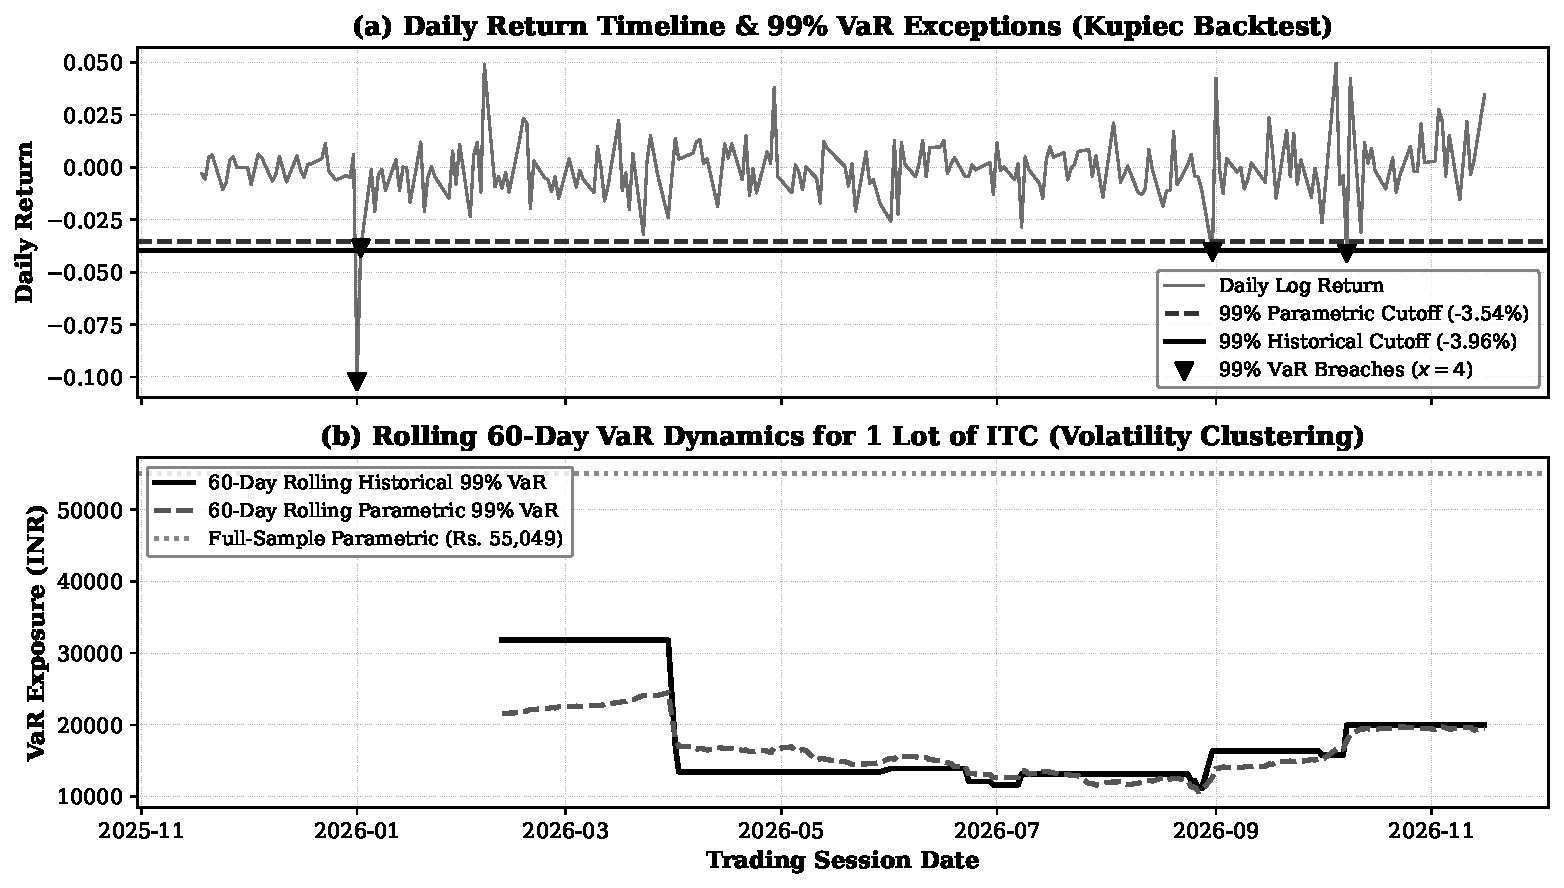
\includegraphics[width=0.95\textwidth, height=4.6cm, keepaspectratio]{figures/fig2_frm_backtest_timeline.pdf}
    \caption{Backtest Timeline and Volatility Clustering Dynamics for ITC Limited (2025--2026). Upper: Daily losses vs. ex-ante $99\%$ $\VaR$ limits. Lower: 60-day rolling annualized volatility driving breach clustering.}
    \label{fig:frm_backtest_timeline}
\end{figure}

\subsection{Empirical Independence and Clustering Findings}

Evaluating the Christoffersen test on our 246 sessions yields critical diagnostic insights:
\begin{itemize}[leftmargin=1.5em, itemsep=1pt, parsep=0pt]
    \item \textbf{99\% Historical Simulation VaR:} $n_{00} = 239$, $n_{01} = 3$, $n_{10} = 3$, $n_{11} = 0 \implies \hat{\pi}_{11} = 0.0$. Test yields $\LR_{\text{ind}} = 0.0744$ ($p = 0.7851$) and combined conditional coverage $\LR_{\text{cc}} = 0.1863$ ($p = 0.9111$). Fully satisfies conditional coverage with zero clustering.
    \item \textbf{99\% Parametric VaR:} $n_{00} = 238$, $n_{01} = 3$, $n_{10} = 3$, $n_{11} = 1 \implies \hat{\pi}_{11} = 25.0\%$. Consequently, $\LR_{\text{ind}} = 4.0758$ ($p = 0.0435$), **rejecting exception independence at the 5\% level** due to a consecutive breach during the February Union Budget announcement period.
\end{itemize}

\clearpage
